\section{Ensamble Methods}
\subsection{Wisdom of Crowd}
\begin{itemize}
    \item Suppose you have a difficult question
    \item Ask many people and aggregate the answer
    \item This might work very well instead of finding the best suited person
\end{itemize}

\subsection{Ensamble}
\begin{itemize}
    \item Wisdom of Crowd can be applied to ML
    \item Instead of finding the best model, aggregate the results of weak models
    \item Aggregate predictions of regressors or classifiers
    \item Might get better accuracy than the best predictor
    \item Ensamble: group of predictors
\end{itemize}

\subsection{Ensamble Method}
\begin{itemize}
    \item Suppose we have many different weak models (better than random)
    \item Get prediction from all of them and take a vote
    \item Class with most votes is the predicted class
    \item Commonly used towards the end of a project
    \item \textbf{Requirement}: enough models / diverse models
\end{itemize}

\subsection{Bagging and Pasting}
\textbf{Bagging (Bootstrap Aggregating)}
\begin{itemize}
    \item Sampling with replacement
    \item Allows data points to be used several times
\end{itemize}
\textbf{Pasting}
\begin{itemize}
    \item Sampling without replacement
\end{itemize}

\subsection{No free lunch theorem}
\textit{No single machine learning algorithm is universally the best-performing algorithm for all problems}

\subsubsection{Out of Bag (oob) Evaluation}
\begin{itemize}
    \item Using Bagging
    \item Some Data Points may not be used at all
    \item Use them for evaluation 
\end{itemize}

\subsubsection{Voting}
\begin{itemize}
    \item Hard voting: Predict the class that gets the most votes
    \item Soft voting (only possible if predictions are probabilities, not classes): Predict the class with the highest class probability, averaged over all classifiers
\end{itemize}
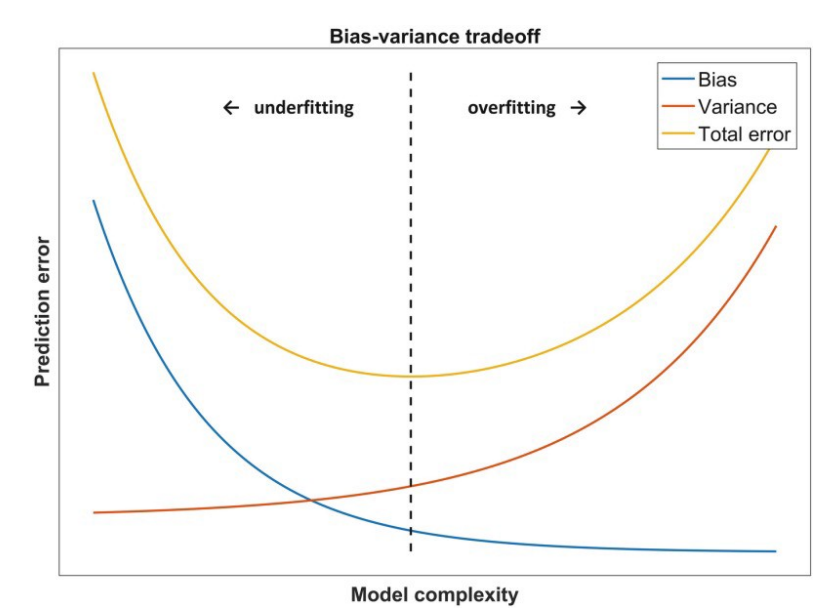
\includegraphics[width=\linewidth]{variance.png}